% Geometry of the second response (@fig-derivation): the consumer's reporting
% rule on the probability scale, and the researcher's evaluation of the same
% thresholds on the utility scale.
%
% Drawn for W = 4.  The cut points are fixed on the utility scale at
% F^{-1}(alpha) = (-0.5, 0.9, 2.3) -- spaced so the abscissa labels clear one
% another -- giving (alpha_1, alpha_2, alpha_3) = (0.1923, 0.6659, 0.9046).
% u* = 0.30, so p = F(u*) = 0.4767, which falls in [alpha_1, alpha_2) and the
% consumer reports y = 2.  S_it = 2, i.e. mubar_it = ln 2, so the right
% panel's ordinates are alpha_w^2 = (0.0370, 0.4435, 0.8183).
%
% Plain TikZ only -- no pgfplots -- so this rebuilds with the same toolchain
% as timing.tex. Rebuild both outputs from this directory with:
%   pdflatex derivation.tex && pdftocairo -svg derivation.pdf derivation.svg
\documentclass[tikz,border=4pt]{standalone}
\usepackage{amsmath,amssymb}
\usetikzlibrary{arrows.meta,calc}

% Cut points on the probability scale, and their images under F^{-1} and F^S.
\def\aone{0.192296} \def\atwo{0.665931} \def\athree{0.904603}
\def\cone{-0.5}     \def\ctwo{0.9}      \def\cthree{2.3}
\def\bone{0.036978} \def\btwo{0.443464} \def\bthree{0.818307}
\def\ustar{0.30}    \def\pit{0.476724}

\def\xmin{-1.7} \def\xmax{4.40} \def\xaxend{4.70}

\begin{document}
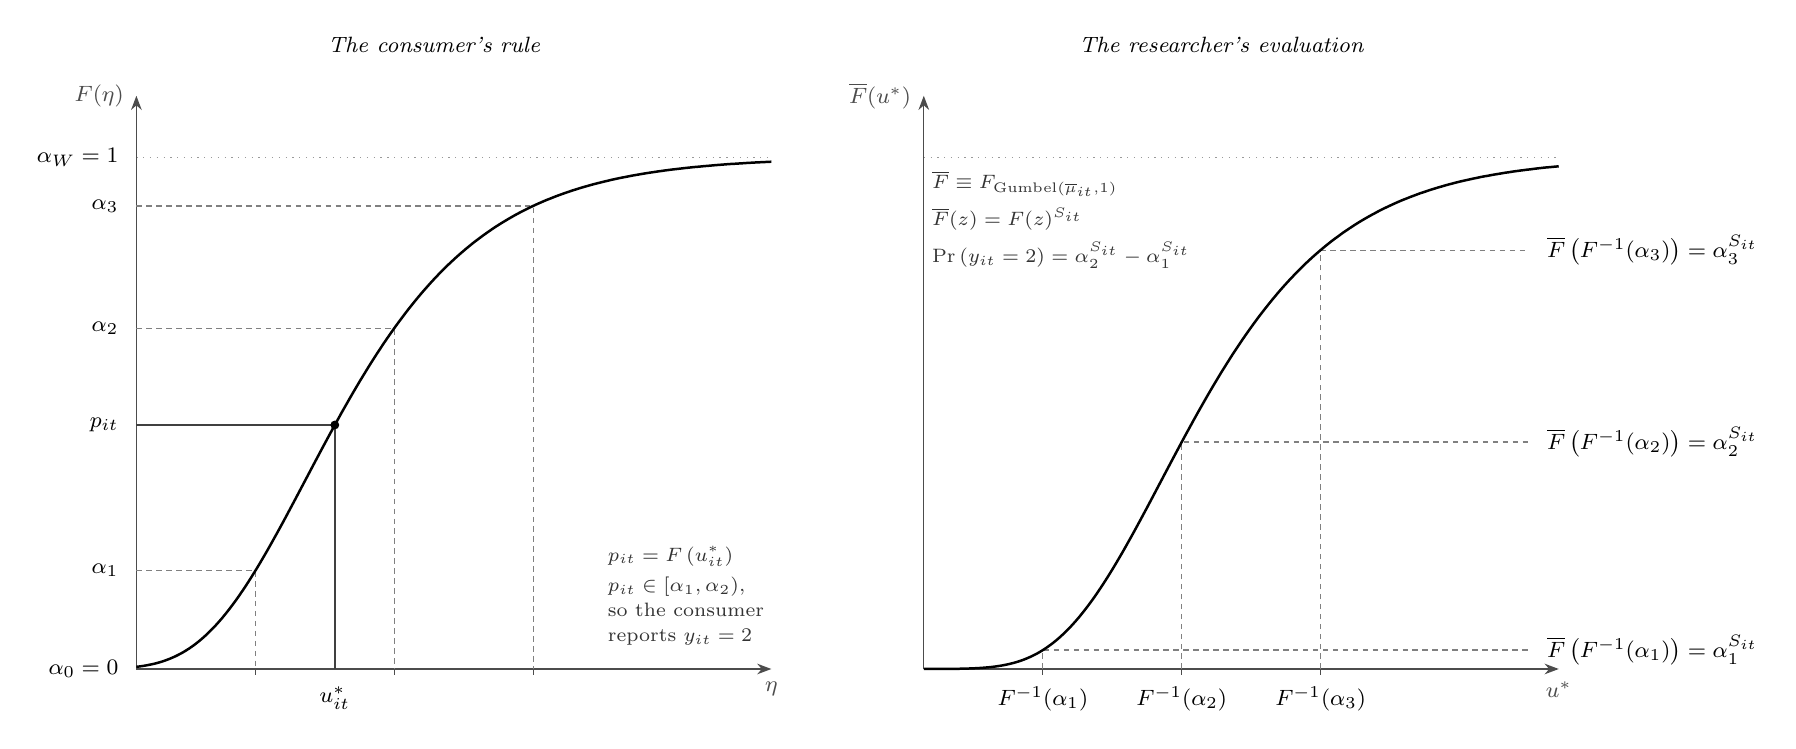
\begin{tikzpicture}[
  font=\footnotesize,
  x=1.26cm, y=6.5cm,
  >={Stealth[length=1.8mm]},
  ax/.style={->, black!70, line width=0.5pt},
  curve/.style={black, line width=0.9pt},
  guide/.style={dashed, black!50, line width=0.45pt, dash pattern=on 2pt off 1.6pt},
  asym/.style={dotted, black!40, line width=0.45pt},
  realized/.style={black!75, line width=0.55pt},
  dot/.style={circle, fill=black, inner sep=0pt, minimum size=3.2pt},
  panel/.style={font=\footnotesize\itshape},
  note/.style={align=left, inner sep=1pt, text=black!80, font=\scriptsize},
]

%% ===================== LEFT PANEL: the consumer's rule =====================
\begin{scope}

  % asymptote at 1 and the axes
  \draw[asym] (\xmin,1) -- (\xaxend,1);
  \draw[ax] (\xmin,0) -- (\xaxend,0) node[below=1pt, black!70] {$\eta$};
  \draw[ax] (\xmin,0) -- (\xmin,1.12) node[left=1pt, black!70] {$F(\eta)$};

  % cut points: across to the curve, then down to the utility scale
  \foreach \a/\c in {\aone/\cone, \atwo/\ctwo, \athree/\cthree} {
    \draw[guide] (\xmin,\a) -- (\c,\a) -- (\c,0);
    \draw[black!70] (\c,0) -- ++(0,-2pt);
  }

  % the realized best utility and the probability it implies: solid, so they
  % read as one draw rather than as two more thresholds
  \draw[realized] (\xmin,\pit) -- (\ustar,\pit) -- (\ustar,0);

  \draw[curve, smooth, samples=180, domain=\xmin:\xaxend]
    plot (\x, {exp(-exp(-\x))});

  \node[dot] at (\ustar,\pit) {};

  % ordinate labels: the cut points, and p_it between alpha_1 and alpha_2
  \node[left=3pt] at (\xmin,0)      {$\alpha_0 = 0$};
  \node[left=3pt] at (\xmin,\aone)  {$\alpha_1$};
  \node[left=3pt] at (\xmin,\pit)   {$p_{it}$};
  \node[left=3pt] at (\xmin,\atwo)  {$\alpha_2$};
  \node[left=3pt] at (\xmin,\athree){$\alpha_3$};
  \node[left=3pt] at (\xmin,1)      {$\alpha_W = 1$};

  % abscissa label
  \node[below=3pt] at (\ustar,0) {$u^*_{it}$};

  % sits in the open wedge right of the last cut point, clear of every guide
  \node[note, anchor=south east] at (4.66,0.04)
    {$p_{it} = F\left( u^*_{it} \right)$\\[3pt]
     $p_{it} \in \left[ \alpha_1, \alpha_2 \right)$,\\[1pt]
     so the consumer\\[1pt]
     reports $y_{it} = 2$};

  \node[panel] at (1.3,1.22) {The consumer's rule};
\end{scope}

%% ================= RIGHT PANEL: the researcher's evaluation =================
\begin{scope}[xshift=10.0cm]

  \draw[asym] (\xmin,1) -- (\xaxend,1);
  \draw[ax] (\xmin,0) -- (\xaxend,0) node[below=1pt, black!70] {$u^*$};
  \draw[ax] (\xmin,0) -- (\xmin,1.12) node[left=1pt, black!70] {$\overline{F}(u^*)$};

  % the same utility-scale thresholds, read off the researcher's CDF
  \foreach \b/\c in {\bone/\cone, \btwo/\ctwo, \bthree/\cthree} {
    \draw[guide] (\c,0) -- (\c,\b) -- (\xmax,\b);
    \draw[black!70] (\c,0) -- ++(0,-2pt);
  }

  \draw[curve, smooth, samples=180, domain=\xmin:\xaxend]
    plot (\x, {exp(-2*exp(-\x))});

  % ordinates on the right, so the long labels do not crowd the panel
  \node[right=3pt] at (\xmax,\bone)   {$\overline{F}\left( F^{-1}(\alpha_1) \right) = \alpha_1^{S_{it}}$};
  \node[right=3pt] at (\xmax,\btwo)   {$\overline{F}\left( F^{-1}(\alpha_2) \right) = \alpha_2^{S_{it}}$};
  \node[right=3pt] at (\xmax,\bthree) {$\overline{F}\left( F^{-1}(\alpha_3) \right) = \alpha_3^{S_{it}}$};

  % abscissae, all on one level now that the cut points are spread
  \node[below=3pt] at (\cone,0)   {$F^{-1}(\alpha_1)$};
  \node[below=3pt] at (\ctwo,0)   {$F^{-1}(\alpha_2)$};
  \node[below=3pt] at (\cthree,0) {$F^{-1}(\alpha_3)$};

  \node[note, anchor=north west] at (-1.65,0.98)
    {$\overline{F} \equiv F_{\text{Gumbel}(\overline{\mu}_{it},1)}$\\[3pt]
     $\overline{F}(z) = F(z)^{S_{it}}$\\[3pt]
     $\Pr\left( y_{it} = 2 \right) = \alpha_2^{S_{it}} - \alpha_1^{S_{it}}$};

  \node[panel] at (1.3,1.22) {The researcher's evaluation};
\end{scope}

\end{tikzpicture}
\end{document}
